\chapter{Gradientni sestop, odvajanje in računski graf}

Večina postopkov, ki jih bomo spoznali in uporabljali pri predmetu o ``odkrivanje znanj iz podatkov'' temelji na modernih pristopih strojnega učenja. Ta, poenostavljeno, gradi modele iz učnih podatkov tako, da pri določeni podani strukturi modela išče njegove parametre tako, da pri tem zadovolji pogoje kriterijske funkcije, ki jo določimo nad učnimi podatki. Zadovoljevanje pogojev tipično pomeni minimizacijo kriterijske funkcije in s tem uporabo optimizacijskih algoritmov. Iz zgrajenih modelov razpoznamo vzorce v podatkih in če so ti razumljivo zapisani ali pa jasno izrisani v nekem grafičnem prikazu lahko modele, in s tem podatke, interpretiramo in iz interpretacij morda odkrijemo nova znanja.

Zgornji odstavek je začetek prvega poglavja nekega predmeta precej preobložen. Do njegovega razumevanja se bomo morali še prebiti. A to ne bomo počeli v tem poglavju. Prejšnji odstavek smo namreč zapisali samo zato, da uvedem pojem ``kriterijske funkcije'' in namignemo, da za neko, lahko enostavno lahko pa zelo kompleksno funkcijo, iščemo njen ``minimum''. Tu se zaenkrat ustavimo in si vse skupaj poglejmo na enostavnem primeru.

\section{Primer}

Začnimo s preprosto funkcijo: 

\[
f(a) = a^2 - 10a + 28
\]

\noindent Želimo poiskali takšno vrednost parametra \( a \), pri kateri ima ta funkcija najnižjo vrednost.

\textbf{Analitična rešitev}. Ker je dana funkcija enostavna, kvadratna, lahko njen minimum poiščemo analitično. Funkcija bo imela ekstrem v točki, kjer je prvi odvod enak nič. Odvajamo našo funkcijo:  

\[
\frac{d}{da} f(a) = 2a - 10
\]

\noindent in njen odvod enačimo z nič:  

\[
2a - 10 = 0
\]

\noindent Rešimo za \( a \):  

\[
a = 5
\]

\noindent Vrednost funkcije v tej točki je:  

\[
f(5) = 5^2 - 10(5) + 28 = 25 - 50 + 28 = 3
\]

\noindent Torej funkcija doseže svoj minimum pri \( a = 5 \), kjer velja \( f(5) = 3 \).  

\textbf{Numerična rešitev}. Poiščimo to rešitev še numerično. Postopek iskanja minimuma bomo pričeli pri neki izbrani vrednosti parametra \( a \), tam izračunali odvod funkcij, in vrednost parametra spremenili v smeri negativnega odvoda, torej $a$ povečali, če bo odvod negativen, ali pa $a$ zmanjšali, če bo odvod pozitiven. 

Razmislimo: pri pozitivnem odvodu funkcije za izbrano vredno parametra $a$ se pri povečanju te vrednosti $a$ vrednost funkcije zveča. Odvod nam namreč pove v katero smer in kako hitro se vrednost funkcije spremeni pri majhni spremembi parametra 
$a$. Zato, če iščemo minimum, moramo vrednost $a$ zmanjšati. Odločiti se moramo seveda za koliko jo bomo zmanjšali, a intuitivno je to prav gotovo odvisno od velikosti odvoda: če pri vrednosti $a$ funkcija hitro narašča, torej je odvod visok, lahko vrednost $a$ popravimo za več kot v primeru, ko je naraščanje zelo počasno in smo morda že prav blizu ekstrema funkcije. Podobno, samo z ravno nasprotnim predznakom, lahko ravnamo ob negativnem odvodu, popravek parametra $a$ pa lahko zapišemo z:
\[
a_{t+1} = a_t - \eta \frac{d}{da} f(a_t)
\]
\noindent kjer je $a_{t+1}$ vrednost parametra po $t$-tem popravku in kjer je $\eta$ korak popravka, v strojnem učenju pa ga bomo imenovali tudi {\em hitrost učenja}. Meta parameter $\eta$ torej določa, kako veliki bodo koraki pri posodabljanju vrednosti parametra. Imenujemo ga {\em meta} ker je parameter naše numerične metode, s katero iščemo rešitev, in torej ne parameter funkcije, ki jo optimiziramo (tem parametrom pravimo samo parameteri, brez predpone ``meta'').

Vse skupaj seveda pričnemo pri neki {\em začetni vrednosti} parametra, $a_0$. Na primer, začnimo z začetno vrednostjo $a_0=6$ in izberimo hitrost učenja $\eta = 0.1$ ter poglejmo, kam vse skupaj vodi:

\begin{enumerate}
\item Izračunamo odvod funkcije pri \( a_0 = 6 \):
\[
\frac{d}{da} f(6) = 2(6) - 10 = 12 - 10 = 2
\]
\noindent in posodobimo vrednost parametra,
\[
a_1 = 6 - 0.1 \times 2 = 6 - 0.2 = 5.8
\]
\item Izračunamo odvod pri novi vrednosti parametra, \( a_1 = 5.8 \):
\[
\frac{d}{da} f(5.8) = 2(5.8) - 10 = 11.6 - 10 = 1.6
\]
\noindent in ponovno posodobimo njegovo vrednost,
\[
a_2 = 5.8 - 0.1 \times 1.6 = 5.8 - 0.16 = 5.64
\]
\item Izračunamo gradient pri \( a_2 = 5.64 \):
\[
\frac{d}{da} f(5.64) = 2(5.64) - 10 = 11.28 - 10 = 1.28
\]
\noindent in posodobimo vrednost parametra $a$, 
\[
a_3 = 5.64 - 0.1 \times 1.28 = 5.64 - 0.128 = 5.512
\]
\end{enumerate}

Smo opazili, da se vrednost odvoda funkcije zmanjšuje, z njo pa tudi zmanjšujejo spremembe parametra $a$? Postopek bi morali seveda nadaljevati, in če je vse tako, kot smo si zamislili, bi se morala vrednost parametra $a$ približati 5. Tam gre tudi odvod funkcije $f(a)$ proti nič in z njo gredo proti nič tudi vrednost popravkov parametra.

Čas je, da tovrstno iskanje minimuma funkcije implementiramo v kodi:

\vspace*{3mm}
\begin{lstlisting}
def f(a):
    return a**2 - 10*a + 28

def df(a):
    return 2*a - 10

a = 6
eta = 0.1
for _ in range(20):
    grad = df(a)
    a = a - eta * grad
    print(f"a = {a:.6f}, f(a) = {f(a):.6f}")
\end{lstlisting}

Pomagali smo si z analitičnim odvodom funkcije, in ga zapisali v funkciji \texttt{df}. Ko program poženemo, se ta hitro približa pravi rešitvi:

\vspace*{3mm}
\begin{lstlisting}
a = 5.800000, f(a) = 3.640000
a = 5.640000, f(a) = 3.409600
a = 5.512000, f(a) = 3.262144
...
a = 5.014412, f(a) = 3.000208
a = 5.011529, f(a) = 3.000133
\end{lstlisting}

Namesto analitičnega zapisa odvoda funkcije lahko tega izračunamo tudi numerično z metodo končnih diferenc, kot smo to storili v spodnji funkciji.
\vspace*{3mm}
\begin{lstlisting}
def df(a, h=0.0001):
    return (f(a + h) - f(a)) / h
\end{lstlisting}

\noindent Tipično je uporaba analitično izračunanega odvoda oziroma gradientov hitrejša in bolj točna ter ni odvisna od uporabe parametra \texttt{h}, katerega vrednost bi morali še določiti (zgoraj smo sicer izbrali privzeto vrednost 0.0001) in ki dejansko vpliva na točnost rezultatov. Zato se bomo od tu dalje delali z analitično izračunanimi odvodi!

\section{Gradientni sestop}

Preden nadaljujemo z (analitičnim) odvajanjem samo zabeležimo in poimenujmo: postopek, ki smo ga zgoraj uporabili za izračun minimuma dane funkcije, se imenuje {\em gradientni sestop}. Ta v vsakem koraku oceni, kako strma je funkcija pri dani vrednosti parametra in nato njegovo vrednost popravi v smeri negativnega odvoda. Pomembno je izbrati ustreen korak popravka $\eta$. Če je prevelika, se nam lahko zgodi, da bomo minimum ``preskočili'', če je premajhna, bo postopek zelo počasen.

Da lahko izvedemo gradientni sestop, moramo poznati odvod funkcije po danem parametru. 
V primeru enega parametra je gradient enak navadnemu odvodu, 
v primeru večparametrske funkcije pa moramo poznati odvode po vseh parametrih. 
Vektorju teh odvodov pravimo gradient in ga označimo z $\nabla f(\boldsymbol{\theta})$, 
kjer je $\boldsymbol{\theta}$ vektor parametrov:

\[
\nabla f(\boldsymbol{\theta}) = 
\left(
\frac{\partial f}{\partial \theta_1},
\frac{\partial f}{\partial \theta_2},
\dots,
\frac{\partial f}{\partial \theta_n}
\right)^T
\]

Tudi gradient funkcije lahko določimo analitično ali numerično z metodo končnih diferenc, a bomo, zaradi enakih razlogov kot pri odvajanju, tudi tu uorabili analitično rešitev. Ker je ročno odvajanje za kompleksne funkcije (beri: kompleksne modele), kot so na primer nevronske mreže, zamudno, se moramo zateči k boljši rešitvi: uporabi programa za odvajanje. Program za strojno odvajanje bomo razvili v naslednjem poglavju, tu pa si poglejmo, kako se problema strojnega odvajanja sploh lotimo, najprej torej ročno.


\section{Računski graf}

Začnimo s primerom in z enostavno funkcijo štirih parametrov:

\[
L(a, b, c, d) = (ab + c) d
\]

Za to funkcijo bi radi izračunali gradient pri vrednostih njenih parametrov \( a = 2 \), \( b = -3 \), \( c = 10 \), \( d = -2 \). Želeli bi torej izračunati sledeče parcialne odvode:
%
\[
\frac{\partial L}{\partial a}, \frac{\partial L}{\partial b}, \frac{\partial L}{\partial c}, \frac{\partial L}{\partial d}.
\]
%
\noindent Z drugimi besedami, želeli bi izračunati gradient funkcije pri danih vrednosti parametrov:
\[
\nabla L = \left( \frac{\partial L}{\partial a}, \frac{\partial L}{\partial b}, \frac{\partial L}{\partial c}, \frac{\partial L}{\partial d} \right)
\]

Najprej si skušajmo olajšati naše računanje odvodov tako, da funkcijo razstavimo in zapišemo z vpeljavo vmesnih spremenljivk, katerih vrednost izračunamo z neko osnovno operacijo (množenje ali seštevanje):

\begin{align*}
e &= ab \\
f &= e + c \\
L &= fd
\end{align*}

Tako zapisano funkcijo lahko sedaj ponazorimo grafično s spodnjim {\em računskim grafom}. V grafično predstavitev smo zapisali tudi (trenutno) vrednost vseh izvedenih spremenljivk, to je spremenljivk $e$ in $f$.

\begin{figure*}
  \centering{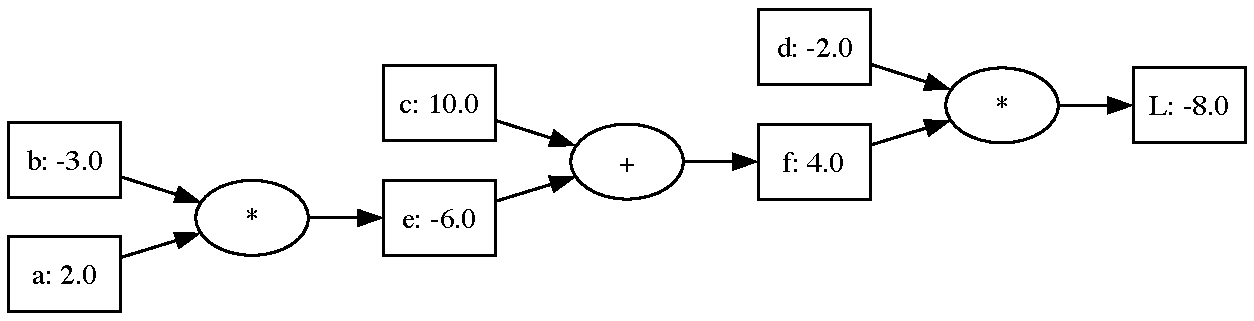
\includegraphics[width=0.9\textwidth]{figs/010-racunski-graf.pdf}}
  \caption[6pt]{}
  \label{fig:racunski-graf}
\end{figure*}

Lotimo se odvajanj. Opazimo, da je naša funkcija $L$ neposredno odvisna od spremenljivk $d$ in $f$, zato je najlažje začeti z odvajanjem po teh spremenljivkah. Najprej za spremenljivko $d$. Zanima nas torej, kako se spremeni vrednost funkcije $L$, če spremenimo vrednost $d$-ja:

\[
\frac{\partial L}{\partial d} = \lim_{h \to 0} \frac{f(d+h) - fd}{h} = \lim_{h \to 0} \frac{fd + fh - fd}{h} = \lim_{h \to 0} \frac{fh}{h} = f
\]
%
\noindent Ker je vrednost \( f = 4 \), je torej gradient funkcije $L$ po spremenljivi (ali parametru) $d$ torej enak:

\[
\frac{\partial L}{\partial d} = f = 4
\]

Na podoben način izračunajma še odvod funkcije \( L \) po spremenljivki \( f \):
\[
\frac{\partial L}{\partial f} = \lim_{h \to 0} \frac{(f+h)d - fd}{h} = \lim_{h \to 0} \frac{fd + hd - fd}{h} = \lim_{h \to 0} \frac{hd}{h} = d
\]
%
\noindent Ker vemo, da je \( d = -2 \), je torej odvod po spremenljivki \( f \) enak:
%
\[
\frac{\partial L}{\partial f} = d = -2
\]

Za izračun odvoda po parametru \( c \) rabimo poseči po verižnem pravilu:

\[
\frac{\partial L}{\partial c} = \frac{\partial L}{\partial f} \frac{\partial f}{\partial c}
\]
%
\noindent kjer je \( \frac{\partial f}{\partial c} \) enak:
%
\[
\frac{\partial f}{\partial c} = \frac{\partial (e+c)}{\partial c} = \lim_{h \to 0} \frac{(e+c+h) - (e+c)}{h} = \lim_{h \to 0} \frac{e+c+h-e-c}{h} = \lim_{h \to 0} \frac{h}{h} = 1
\]
%
\noindent Ker smo že izračunali \( \frac{\partial L}{\partial f} = d = -2 \), je torej:

\[
\frac{\partial L}{\partial c} = d \times 1 = -2
\]

Podobno izračunamo parcialni odvod po spremenljivki e, ki bo prav tako enak -2. Ostane name še izračun parcialnih odvodov po spremenljivkah a in b. Začnimo s spremenljivko a:

\[
\frac{\partial L}{\partial a} = \frac{\partial L}{\partial e} \frac{\partial e}{\partial a}
\]

Odvod \( \frac{\partial L}{\partial e} \) poznamo, enak je -2, \( \frac{\partial e}{\partial a} \) pa izračunajmo:

\[
\frac{\partial e}{\partial a} = \frac{\partial (ab)}{\partial a} = \lim_{h \to 0} \frac{(a+h)b - ab}{h} = \lim_{h \to 0} \frac{ab + hb - ab}{h} = \lim_{h \to 0} \frac{hb}{h} = b
\]

Ker je \( b = -3 \) in \( \frac{\partial L}{\partial e} = -2 \), je \( \frac{\partial L}{\partial a} \) torej enak 6. Podobno bi lahko izračunali še, da je \( \frac{\partial L}{\partial b} = -4 \). 

Zgornje računanje ``na roke'' je malce zamudno in pisci tega besedila vedo, da imajo opravka z bralci, ki vse to dobro razumejo in znajo. A smu to samo želeli izpostaviti, da nam pri računanju parcialnih odvodov lahko močno koristi, če funkcijo, ne glede na to, kako kompleksna je, ponazorimo z računskim grafom, ki tipično uporablja neke osnovne in enostavno odvedljive operacije, ter odvode potem računamo vzvratno z verižnim pravilom. 

Spoznali smo tudi, da ko imamo v računskih grafih opravka z vsotami,  ``skopiramo'' vrednost odvoda od staršev vozlišča, pri množenju pa ta odvod pomnožimo še z vrednostjo sosednjega (sestrskega) vozlišča. Paziti sicer moramo pri funkcijah, kjer je staršev določenega vozlišča več: tam bomo morali vplive na starše vozlišča prištevati. Vse to, torej postopek odvajanja z uporabo računskega grafa, pa nam bo zelo prav prišel v naslednjem poglavju, ko bomo sestavljali kodo za strojno odvajanje.